\subsection{Miller}
Il \emph{miller} è il componente che simula la fresatura vera e propria, verificando dove e come l'utensile della macchina compenetra il blocco di materiale, determinando la porzione da rimuovere e decidendo se sia o meno necessario attivare il getto d'acqua di pulitura.

Il prodotto da lavorare (classe \code{Stock}) e l'utensile (classe \code{Cutter}) sono i principali attori di questo modulo. Per gestire in maniera efficiente il processo di erosione lo stock è stato modellato con una particolare struttura dati chiamata \emph{octree}. Un octree è un albero di arietà 8 ---in questo caso, non bilanciato--- che, come si evince dalla figura \ref{fig:octree_explanation}, permette di segmentare uno spazio tridimensionale in regioni via via più piccole man mano che la aumenta la profondità. Ogni foglia rappresenta quindi un parallelepipedo di volume, detto \emph{voxel}, e su di essa è salvato un valore che identifica quali vertici sono stati asportati dal cutter e quali, invece, sono ancora presenti. Per motivi di performance a ciò si aggiungono le informazioni necessarie a calcolare le coordinate dei vertici stessi ed un collegamento alle strutture adibite alla visualizzazione grafica del blocco, come spiegato nella sezione \ref{sec:modules_mesher}.
\begin{figure}[htp]
	\centering
	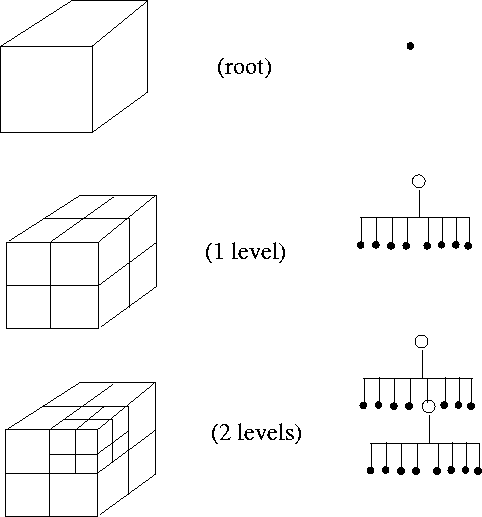
\includegraphics[width=.75\textwidth]{img/octree_explanation}
	\caption{Suddivisione dello spazio tridimensionale tramite albero octree. {\footnotesize (fonte immagine: \url{http://www.forceflow.be/wp-content/uploads/2012/04/octree1.gif})}}
	\label{fig:octree_explanation}
\end{figure}

All'interno del modulo di milling il cutter è caratterizzato da due soli parametri: una \emph{funzione di distanza} e una \emph{bounding box}. La funzione di distanza, descritta nell'equazione \eqref{equ:distance_function} indica se un punto dello spazio è interno o esterno all'utensile: nel caso sia interno, significa che è stato asportato.
\begin{equation} \label{equ:distance_function}
	distance(P) = 
		\begin{cases}
			< 0 & \text{se $P$ è esterno al cutter} \\
			\geq 0 & \text{se $P$ è interno al cutter}
		\end{cases}
	\qquad \text{ dove } P \in \mathbb{R}^3
\end{equation}
L'ingombro del cutter viene modellato attraverso un parallelepipedo orientato. La scelta di questa forma è dovuta al fatto che anche i voxel che costituiscono lo stock sono dei parallelepipedi: il problema dell'intersezione tra box è molto studiato in letteratura, e sono stati individuati algoritmi efficienti per questo tipo di verifica. L'orientamento, invece, serve a poter definire le più piccole dimensioni possibili tali da contenere il cutter: ciò permette di eseguire dei test di intersezione meno rapidi ma anche più accurati.

\subsubsection{Il processo di erosione.}
Per ogni ``mossa'' letta da file, il \emph{miller} converte le due rototraslazioni in una isometria tridimensionale del cutter nei confronti del sistema di riferimento del prodotto. L'algoritmo attraversa quindi l'octree per individuare tutti e soli i voxel che intersecano il volume di riferimento dello stesso cutter: i rami da percorrere sono scelti in base a diverse funzioni di intersezione che diventano via via meno precise, ma più veloci, via via che aumenta la profondità e, di conseguenza, il numero di voxel da analizzare. Giunto ad una foglia dell'albero, l'algoritmo ne enumera i vertici e, per ognuno di essi, invoca la funzione $distance$ del cutter: così facendo si marcano i punti interni alla superficie di taglio che, da quel momento in avanti, verranno considerati erosi.
Le foglie rimaste prive di vertici vengono quindi eliminate, mentre per le altre, se la profondità massima non è ancora stata raggiunta, l'algoritmo effettua una divisione in otto parti del volume di competenza, aggiungendo un nuovo livello all'albero. Come scelta progettuale si è deciso di non condividere i vertici comuni tra voxel contigui in quanto il concetto di vicinanza spaziale non viene modellato bene dalla struttura octree, soprattutto se sbilanciata. Il costo computazionale necessario a recuperare i voxel ``vicini'', infatti, sarebbe stato superiore ai vantaggi portati dalla condivisione dei vertici stessi. Al termine di ogni mossa, il \emph{miller} conteggia la quantità di materiale eroso e non ancora pulito e decide se attivare o meno il getto d'acqua: la scelta viene presa tramite una funzione a doppia soglia, caratterizzata da un ``rate di pulitura'', cioè dal volume di detriti che l'acqua riesce a pulire per ogni mossa.

Mostrare a video lo stato dell'erosione comporta uno scambio di informazioni tra \emph{miller} e \emph{mesher} in quanto questi due algoritmi operano in modo indipendente e con diversi tempi di elaborazione. Per gestire in maniera efficiente l'accesso concorrente ai dati, ogniqualvolta una foglia viene cancellata il \emph{miller} la inserisce in una lista opportuna mentre, per le foglie aggiunte o modificate, il percorso da esse alla radice viene evidenziato. Così facendo il processo di \emph{meshing}, dopo aver acquisito il controllo esclusivo dell'octree, potrà ricavare rapidamente tutte e sole le foglie modificate dalla sua ultima visita. Per impedire che il processo di \emph{milling} possa subire starvation dal \emph{mesher}, quest'ultimo viene attivato al più al termine di ogni mossa letta da file e, comunque, non più di 30 volte al secondo: nei casi reali il tempo di attesa forzata del \emph{miller} è ridotto in quanto, un ciclo di rendering impiega molto più tempo della simulazione di una singola posizione e quest'ultima è più lenta dell'attraversamento dell'albero sui percorsi evidenziati\footnote{I rapporti tra le durate delle operazioni indicate variano di molto in base alla profondità massima dell'albero e alla ``mobilità'' dell'utensile, ovvero al numero di voxel modificati ad ogni iterazione.}.

\subsubsection{Miglioramenti tentati e sviluppi futuri.}
Il processo di \emph{milling} è frutto di più riscritture successive, ognuna delle quali ha sperimentato un modo diverso per rendere più efficiente e veloce l'algoritmo. Il primo approccio scorreva l'albero per livelli sfruttando una coda come struttura dati di appoggio in cui inserire i nodi da analizzare. L'idea di fondo era facilitare la successiva parallelizzazione dell'algoritmo in cui vari thread avrebbero usato la coda per gestire i nodi da controllare, così come mostrato in figura \ref{fig:queue_parallel}.
\begin{figure}[htp]
	\centering
	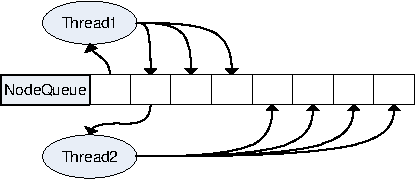
\includegraphics[width=.5\textwidth]{img/queue_parallel}
	\caption{Schematizzazione della prima idea di algoritmo parallelo che risolve il milling.}
	\label{fig:queue_parallel}
\end{figure}

Affrontare una simile strada avrebbe comportato un uso meno efficiente della memoria: l'inserimento dei nodi in una struttura dati in rapida espansione avrebbe comportato molti più accessi in RAM rispetto ad una semplice visita \emph{depth-first} in quanto la gerarchia di cache degli attuali elaboratori non sarebbe stata sfruttata appieno. La speranza era che il parallelismo riuscisse a sopperire a questo problema strutturale e, anzi, ad essere più rapido nell'esecuzione. Questo purtroppo non è avvenuto e, dai confronti con le implementazioni di altri colleghi, le prestazioni risultavano molto inferiori. Le ipotesi sulle motivazioni di questo ``fallimento'' sono state molteplici, ma la più plausibile risiede nell'aver scelto un approccio errato alla parallelizzazione, che male si adatta alla particolare struttura del problema: i nodi che devono venir analizzati sono molti ma, il lavoro da compiere su ognuno di essi è poco, per cui l'impianto necessario a gestire i thread introduce un overhead troppo elevato.

L'esperienza così maturata ha permesso di individuare un approccio migliore nella parallelizzazione del problema, analizzando l'octree attraverso il pattern Fork-Join\footnote{\url{http://www.oracle.com/technetwork/articles/java/fork-join-422606.html}} congiuntamente a uno thread-pool che permetta il \emph{work-stealing}. Così facendo si conservano tutti i vantaggi della visita \emph{depth-first}, senza relegare i thread all'analisi di singoli nodi, e beneficiando sia della possibilità di scrivere codice ricorsivo che di un processing embarassingly parallel.

Purtroppo per carenze di tempo e per la mancanza di librerie che implementano questo paradigma, si è optato per la classica versione ricorsiva. Questa risulta essere la più performante in single-thread ma, dal punto di vista dello spazio occupato, l'implementazione potrebbe essere ulteriormente migliorata, sfruttando i vantaggi offerti dalla ricorsione: attualmente, per esempio, ogni nodo dell'albero contiene un riferimento al padre, retaggio delle vecchie realizzazioni; questo puntatore può essere rimosso mantenendo comunque la possibilità di ``risalire'' la struttura dati durante il completamento delle chiamate ricorsive.

